\documentclass[12pt,hyperref,a4paper,UTF8]{ctexart}
\usepackage{HDUReport}
\usepackage{listings}
\usepackage{xcolor}
\usepackage{graphicx}
\usepackage{setspace}
\usepackage{float}


\usepackage[UTF8]{ctex} % 支持中文,如果您用xeCJK或CJK请相应调整
\usepackage[T1]{fontenc} % 推荐,改善字体编码和下划线等字符的处理
\usepackage{lmodern}     % 推荐,与T1结合使用效果更佳

\setstretch{1.5} % 设置全局行距为1.5倍

\usepackage{enumitem} % 载入enumitem包以便自定义列表环境
\setlist[itemize]{itemsep=0pt, parsep=0pt} % 设置itemize环境的项目间距和段落间距

\setmainfont{Times New Roman} % 英文正文为Times New Roman


\usepackage{tikz}
\usetikzlibrary{shapes.geometric, arrows}
\usetikzlibrary{positioning, arrows.meta}
\usetikzlibrary{calc}
\usetikzlibrary{fit}


%Verilog 代码样式设置
\lstdefinelanguage{Verilog}{
    keywords=[1]{module, input, output, wire, reg, assign, always, if, else, endmodule, begin, end, case, endcase, parameter},
    keywords=[2]{posedge, negedge, clk, rst, logic},
    keywordstyle=[1]\color{blue}\bfseries,
    keywordstyle=[2]\color{teal}\bfseries,
    identifierstyle=\color{black},
    commentstyle=\color{gray}\itshape,
    stringstyle=\color{red}\ttfamily,
    morecomment=[l]{//},
    morecomment=[s]{/*}{*/},
    morestring=[b]",
    sensitive=true
}

\lstset{
    basicstyle=\ttfamily\footnotesize,
    numbers=left,
    numberstyle=\tiny\color{gray},
    stepnumber=1,
    numbersep=5pt,
    tabsize=4,
    showspaces=false,
    showstringspaces=false,
    breaklines=true,
    frame=single,
    language=Verilog
}

%封面页设置
{   
    %标题
    \title{ 
        \vspace{1cm}
        \heiti \Huge \textbf{电子信息技术虚拟仿真实验报告} \par
        \vspace{1cm} 
        \heiti \Large {\underline{基于Nios II 实现多类型LCD屏幕彩条显示}   } 
        \vspace{1cm}
    
    }

    \author{
        \vspace{0.5cm}
        \kaishu\Large 学院\ \dlmu[9cm]{卓越学院} \\ %学院
        \vspace{0.5cm}
        \kaishu\Large 学号\ \dlmu[9cm]{23040447} \\ %班级
        \vspace{0.5cm}
        \kaishu\Large 姓名\ \dlmu[9cm]{陈文轩} \qquad  \\ %学号
        \vspace{0.5cm}
        \kaishu\Large 专业\ \dlmu[9cm]{智能硬件与系统(电子信息工程)} \qquad \\ %姓名 
        \vspace{0.5cm}
        \kaishu\Large 指导教师\ \dlmu[9cm]{徐魁文、吴岩} \qquad \\ %姓名 
    }
        
    \date{\today} % 默认为今天的日期,可以注释掉不显示日期
}
%%------------------------document环境开始------------------------%%
\begin{document}

%%-----------------------封面--------------------%%
\cover
\thispagestyle{empty} % 首页不显示页码
%%------------------摘要-------------%%
%\newpage
%\begin{abstract}




%\end{abstract}

%\thispagestyle{empty} % 首页不显示页码

%%--------------------------目录页------------------------%%
% \newpage
% \tableofcontents
% \thispagestyle{empty} % 目录不显示页码

%%------------------------正文页从这里开始-------------------%
\newpage
\setcounter{page}{1} % 让页码从正文开始编号

%%可选择这里也放一个标题
%\begin{center}
%    \title{ \Huge \textbf{{标题}}}
%\end{center}



%%------------------摘要-------------%%
\newpage
\begin{abstract}
本实验通过 Qsys 系统集成工具,利用 Altera 提供的 IP 核,搭建了一个简单的 SOPC 系统,并设计了 IP 核之间的互联逻辑。
实验中将 Nios II 嵌入式软核处理器部署在 EP4CE10F17C8 正点原子开发板上,
结合 SDRAM 、LCD 屏幕等硬件模块与Avalon-MM突发传输控制、SDRAM控制器、SDRAM桥控制器等软件模块,完成了软硬件协同设计。
最后通过嵌入式 C 程序的开发,实验实现了兼容驱动多种类型 LCD 屏幕的功能,并能够显示指定颜色和宽度的彩条。



关键词:\textbf{LCD屏幕,Qsys开发,NiosII软核}
\end{abstract}

\thispagestyle{empty} % 摘要页不显示页码
\newpage

\section{引言}

当今世界,电子信息技术以极快的速度在发展,各种各样的电子产品在我们的日常生活中都变得必不可少。比如手机、电脑等等。这些产品的设计开发,当然少不了最基础的LCD显示器。LCD显示器作为人机交互的关键窗口,其驱动与控制技术的实现至关重要。随着可编程逻辑器件(FPGA)技术的成熟,其并行处理能力、高集成度和可重构性使其在图像处理和显示控制领域展现出巨大潜力。特别是基于FPGA的片上可编程系统(SOPC)技术,允许设计者将处理器核、存储器接口、外设接口等集成在单一芯片上,为复杂的嵌入式显示系统提供了高效灵活的解决方案。

在此背景下,本实验旨在探索和实践一种基于SOPC的LCD显示控制系统设计方法。实验通过Altera公司的Qsys系统集成工具,利用其提供的IP核,在EP4CE10F17C8 FPGA开发板上搭建了一个包含Nios II嵌入式软核处理器的SOPC系统。该系统整合了SDRAM、LCD屏幕等关键硬件模块,并利用Avalon-MM突发传输控制、SDRAM控制器及桥控制器等软件模块,实现了高效的软硬件协同工作。通过开发嵌入式C程序,本实验成功实现了对多种类型LCD屏幕的兼容驱动,并能在屏幕上显示指定颜色和宽度的彩条。这一实践不仅完整展示了基于FPGA的嵌入式系统设计全流程,也为软硬件协同开发提供了宝贵的实践经验,为未来构建更为复杂的嵌入式系统奠定了坚实基础。


\section{系统总体硬件设计}


\begin{figure}[H] % [H] 表示强制当前位置插入
        \centering
        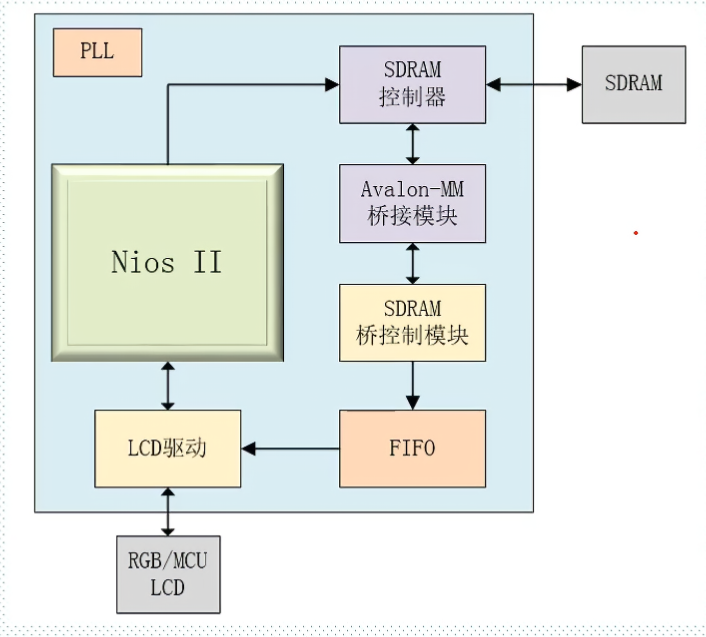
\includegraphics[width=1\textwidth]{figures/001.png} % 调整宽度为文本宽度的 80%
        \caption{系统框图} %图片标题
        \label{fig:example} % 图片标签,用于引用
\end{figure}

该系统框图展示了一个基于FPGA的嵌入式系统,其核心目标是驱动一个LCD显示屏显示内容。图中浅蓝色背景框内的部分代表了在FPGA芯片内部实现的逻辑和组件,框外的SDRAM和RGB/MCU LCD是外部物理器件。

\subsection*{各模块功能及连接关系解释}

\subsubsection*{1. Nios II 处理器 (Nios II)}
\begin{itemize}
    \item \textbf{功能:} 这是系统的“大脑”,一个软核嵌入式处理器。它负责运行用户编写的C程序,执行控制逻辑,准备要显示的数据,以及配置其他外设(如LCD驱动模块)。
    \item \textbf{连接:}
    \begin{itemize}
        \item 连接到 \textbf{LCD驱动模块}:Nios II通过控制总线向LCD驱动模块发送命令和配置参数(例如,要显示的颜色、彩条宽度、启动显示等)。
        \item 连接到 \textbf{Avalon-MM 桥接模块}:Nios II通过Avalon总线访问系统中的其他IP核,最主要的是访问SDRAM。它可以向SDRAM中写入要显示的图像数据,或者从中读取程序代码和运行时数据。
        \item (隐含连接) 通常由 \textbf{PLL} 提供工作时钟。
    \end{itemize}
\end{itemize}

\subsubsection*{2. PLL (Phase-Locked Loop, 锁相环)}
\begin{itemize}
    \item \textbf{功能:} 时钟管理单元。它接收外部时钟信号,并根据系统需求生成不同频率、相位的稳定时钟信号,供FPGA内部的各个模块使用,如Nios II处理器、SDRAM控制器等。
    \item \textbf{连接:}
    \begin{itemize}
        \item (隐含连接) 为Nios II、SDRAM控制器以及其他FPGA内部逻辑提供时钟。
        \item 图中明确指向 \textbf{SDRAM控制器},表明它为SDRAM控制器提供精确的工作时钟。
    \end{itemize}
\end{itemize}

\subsubsection*{3. SDRAM 控制器 (SDRAM Controller)}
\begin{itemize}
    \item \textbf{功能:} 这是一个IP核,负责管理与外部SDRAM芯片的物理接口和通信协议。它处理SDRAM的初始化、刷新、读写时序等复杂操作,将来自Avalon总线的简单读写请求转换为SDRAM能理解的命令。
    \item \textbf{连接:}
    \begin{itemize}
        \item 连接到外部 \textbf{SDRAM} 芯片:进行物理层的数据交换。
        \item 连接到 \textbf{Avalon-MM 桥接模块}:作为Avalon总线的从设备,接收来自Nios II或SDRAM桥控制模块的读写请求。
        \item 接收来自 \textbf{PLL} 的时钟信号。
    \end{itemize}
\end{itemize}

\subsubsection*{4. 外部 SDRAM (Synchronous Dynamic Random-Access Memory)}
\begin{itemize}
    \item \textbf{功能:} 大容量的动态随机存储器,用作系统的主内存。在本系统中,它主要用于存储LCD显示的帧缓冲数据(即屏幕上每个像素的颜色信息),也可能存储Nios II处理器的程序代码和运行时数据。
    \item \textbf{连接:} 与FPGA内部的 \textbf{SDRAM控制器} 相连。
\end{itemize}

\subsubsection*{5. Avalon-MM 桥接模块 (Avalon-MM Bridge Module)}
\begin{itemize}
    \item \textbf{功能:} Avalon Memory-Mapped (Avalon-MM) 是一种片上总线标准。这个桥接模块是系统总线的核心组件,用于连接不同的Avalon主设备(如Nios II、SDRAM桥控制模块)和从设备(如SDRAM控制器)。它负责地址译码、数据通路切换和总线仲裁。
    \item \textbf{连接:}
    \begin{itemize}
        \item 连接到 \textbf{Nios II} (作为主设备)。
        \item 连接到 \textbf{SDRAM 控制器} (作为从设备)。
        \item 连接到 \textbf{SDRAM 桥控制模块} (作为主设备,用于访问SDRAM)。
    \end{itemize}
\end{itemize}

\subsubsection*{6. SDRAM 桥控制模块 (SDRAM Bridge Control Module)}
\begin{itemize}
    \item \textbf{功能:} 这个模块很可能是一个专用的数据搬运控制器,例如DMA(Direct Memory Access)控制器,专门负责高效地从SDRAM中读取显示数据,并将其送往显示流水线的下一级(FIFO)。它能以突发模式高速读取SDRAM中的数据,减轻Nios II处理器的负担。
    \item \textbf{连接:}
    \begin{itemize}
        \item 连接到 \textbf{Avalon-MM 桥接模块}:作为Avalon主设备,发起对SDRAM的读操作。
        \item 连接到 \textbf{FIFO}:将从SDRAM读取到的显示数据写入FIFO。
    \end{itemize}
\end{itemize}

\subsubsection*{7. FIFO (First-In, First-Out) 缓冲器}
\begin{itemize}
    \item \textbf{功能:} 先入先出缓冲存储器。它在数据速率可能不匹配的两个模块之间起到缓冲作用。在此,它用于缓冲从SDRAM高速读取的显示数据,然后LCD驱动模块可以按照自己的固定速率从中读取数据,平滑数据流。
    \item \textbf{连接:}
    \begin{itemize}
        \item 接收来自 \textbf{SDRAM 桥控制模块} 的数据。
        \item 向 \textbf{LCD驱动模块} 输出数据。
    \end{itemize}
\end{itemize}

\subsubsection*{8. LCD驱动模块 (LCD Driver)}
\begin{itemize}
    \item \textbf{功能:} 这是一个IP核,负责生成驱动LCD屏幕所需的特定时序信号(如行同步、场同步、像素时钟)和数据信号。它从FIFO中读取像素数据,按照LCD的时序要求将其输出到外部LCD屏幕。
    \item \textbf{连接:}
    \begin{itemize}
        \item 接收来自 \textbf{FIFO} 的像素数据。
        \item 接收来自 \textbf{Nios II} 的控制/配置信号。
        \item 输出驱动信号到外部 \textbf{RGB/MCU LCD}。
        \item 通过SDRAM桥接、Avalon-MM桥接、SDRAM控制器,读取LCD的设置信息
    \end{itemize}
\end{itemize}

\subsubsection*{9. RGB/MCU LCD (外部LCD显示屏)}
\begin{itemize}
    \item \textbf{功能:} 物理显示设备。它接收来自LCD驱动模块的RGB数据信号和控制信号,并将图像显示出来。
    \item \textbf{连接:} 与FPGA内部的 \textbf{LCD驱动模块} 相连。
\end{itemize}

\subsection*{数据流总结 (以显示为例)}
\begin{enumerate}
    \item \textbf{数据准备:} Nios II 处理器计算或准备好要显示的彩条数据(像素颜色信息),并将这些数据通过 \textbf{Avalon-MM 桥接模块} 写入到外部 \textbf{SDRAM} 的帧缓冲区中。
    \item \textbf{数据读取与传输:}
    \begin{itemize}
        \item \textbf{SDRAM 桥控制模块} 被触发后,通过 \textbf{Avalon-MM 桥接模块} 和 \textbf{SDRAM 控制器},以突发模式从 \textbf{SDRAM} 中高速读取帧缓冲数据。
        \item 读取到的数据被写入 \textbf{FIFO} 缓冲器。
    \end{itemize}
    \item \textbf{数据显示:}
    \begin{itemize}
        \item \textbf{LCD驱动模块} 按照其工作时钟和LCD的刷新率,从 \textbf{FIFO} 中读取像素数据。
        \item 同时,\textbf{LCD驱动模块} 生成符合LCD接口规范的控制时序信号。
        \item 像素数据和控制信号一起被发送到外部 \textbf{RGB/MCU LCD},最终在屏幕上显示出彩条。
    \end{itemize}
\end{enumerate}

\subsection*{控制流总结}
\begin{itemize}
    \item \textbf{Nios II} 控制整个流程的启动、配置LCD驱动参数(如分辨率、颜色模式、彩条宽度等)、管理SDRAM中的数据等。
    \item \textbf{PLL} 提供稳定的时钟,确保各模块同步协调工作。
    \item 各个\textbf{桥接模块}和\textbf{控制器}则根据Nios II的指令或预设逻辑,自动完成数据在不同接口和存储器之间的传输。
\end{itemize}

该系统体现了SOPC设计的典型特点——软硬件协同工作:Nios II负责灵活的控制和算法处理(软件层面),而FPGA内部的专用硬件IP核(如SDRAM控制器、SDRAM桥控制模块、LCD驱动)负责高速、实时的信号处理和数据传输(硬件层面)。




\section{系统总体软件设计}


\begin{figure}[H] % [H] 表示强制当前位置插入
        \centering
        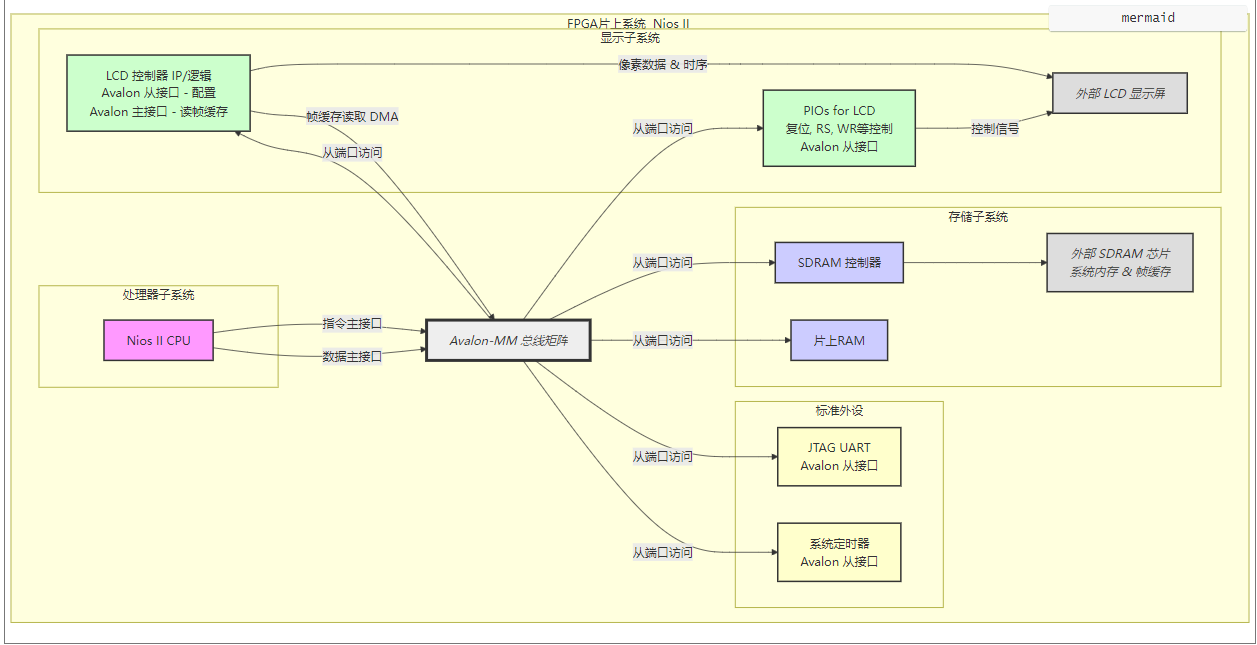
\includegraphics[width=1\textwidth]{figures/002.png} % 调整宽度为文本宽度的 80%
        \caption{系统框图} %图片标题
        \label{fig:example} % 图片标签,用于引用
\end{figure}

\section{系统软件设计与实现}

本实验的软件设计主要围绕 Nios II 处理器的嵌入式 C 程序开发展开,核心目标是通过程序控制 SDRAM 中的显存数据,实现 LCD 屏幕的彩条显示功能。以下是软件设计的主要内容和实现过程。

\subsection{软件功能概述}

软件部分的主要功能包括:
\begin{itemize}
    \item 初始化 LCD 显示屏,配置其分辨率、颜色模式等参数。
    \item 将彩条数据写入 SDRAM 的显存区域,按照屏幕的高度分为五个等宽区域,分别显示红色、白色、黑色、绿色和蓝色。
    \item 刷新数据缓存,确保 SDRAM 中的数据能够正确传输到 LCD 屏幕进行显示。
\end{itemize}

\subsection{代码实现分析}

以下是代码的主要实现步骤:

\subsubsection*{1. LCD 初始化}
通过调用 \lstinline|MY_LCD_Init()| 函数完成 LCD 的初始化,配置屏幕的分辨率和方向等参数。LCD 的宽度和高度信息存储在全局变量 \lstinline|lcdgui| 中,便于后续操作。

\subsubsection*{2. 显存地址分配}
显存的起始地址通过以下代码定义:
\begin{lstlisting}[language=C]
alt_u16 *ram_disp = (alt_u16 *)(SDRAM_BASE + SDRAM_SPAN - 2049000);
\end{lstlisting}
该地址位于 SDRAM 的末尾,用于存储 LCD 显示的像素数据。

\subsubsection*{3. 彩条数据写入}
通过双重循环遍历屏幕的每个像素点,根据其所在的高度范围,将对应的颜色值写入显存:
\begin{itemize}
    \item 红色:高度范围为屏幕的前 1/5。
    \item 白色:高度范围为屏幕的 1/5 到 2/5。
    \item 黑色:高度范围为屏幕的 2/5 到 3/5。
    \item 绿色:高度范围为屏幕的 3/5 到 4/5。
    \item 蓝色:高度范围为屏幕的最后 1/5。
\end{itemize}
颜色值通过 16 位 RGB565 格式表示,例如红色为 \lstinline|0xf800|,绿色为 \lstinline|0x07e0|,蓝色为 \lstinline|0x001f|。

\begin{lstlisting}[language=C]
for(i = 0; i < lcdgui.width; i++) {
    for(j = 0; j < lcdgui.height; j++) {
        if(j < lcdgui.height / 5)
            *(ram_disp++) = 0xf800; // 红色
        else if(j < (lcdgui.height / 5 * 2))
            *(ram_disp++) = 0xffff; // 白色
        else if(j < (lcdgui.height / 5 * 3))
            *(ram_disp++) = 0x0;    // 黑色
        else if(j < (lcdgui.height / 5 * 4))
            *(ram_disp++) = 0x07e0; // 绿色
        else
            *(ram_disp++) = 0x001f; // 蓝色
    }
}
\end{lstlisting}

\subsubsection*{4. 数据缓存刷新}
在数据写入 SDRAM 后,通过调用 \lstinline|alt_dcache_flush_all()| 刷新数据缓存,确保数据能够正确传输到 LCD 屏幕。

\subsection{运行结果}

程序运行后,LCD 屏幕按照预期显示五种颜色的彩条,每种颜色占屏幕高度的 1/5,依次为红色、白色、黑色、绿色和蓝色。该功能验证了系统软硬件协同设计的正确性和可靠性。

\section{调试结果}


\begin{figure}[H] % [H] 表示强制当前位置插入
        \centering
        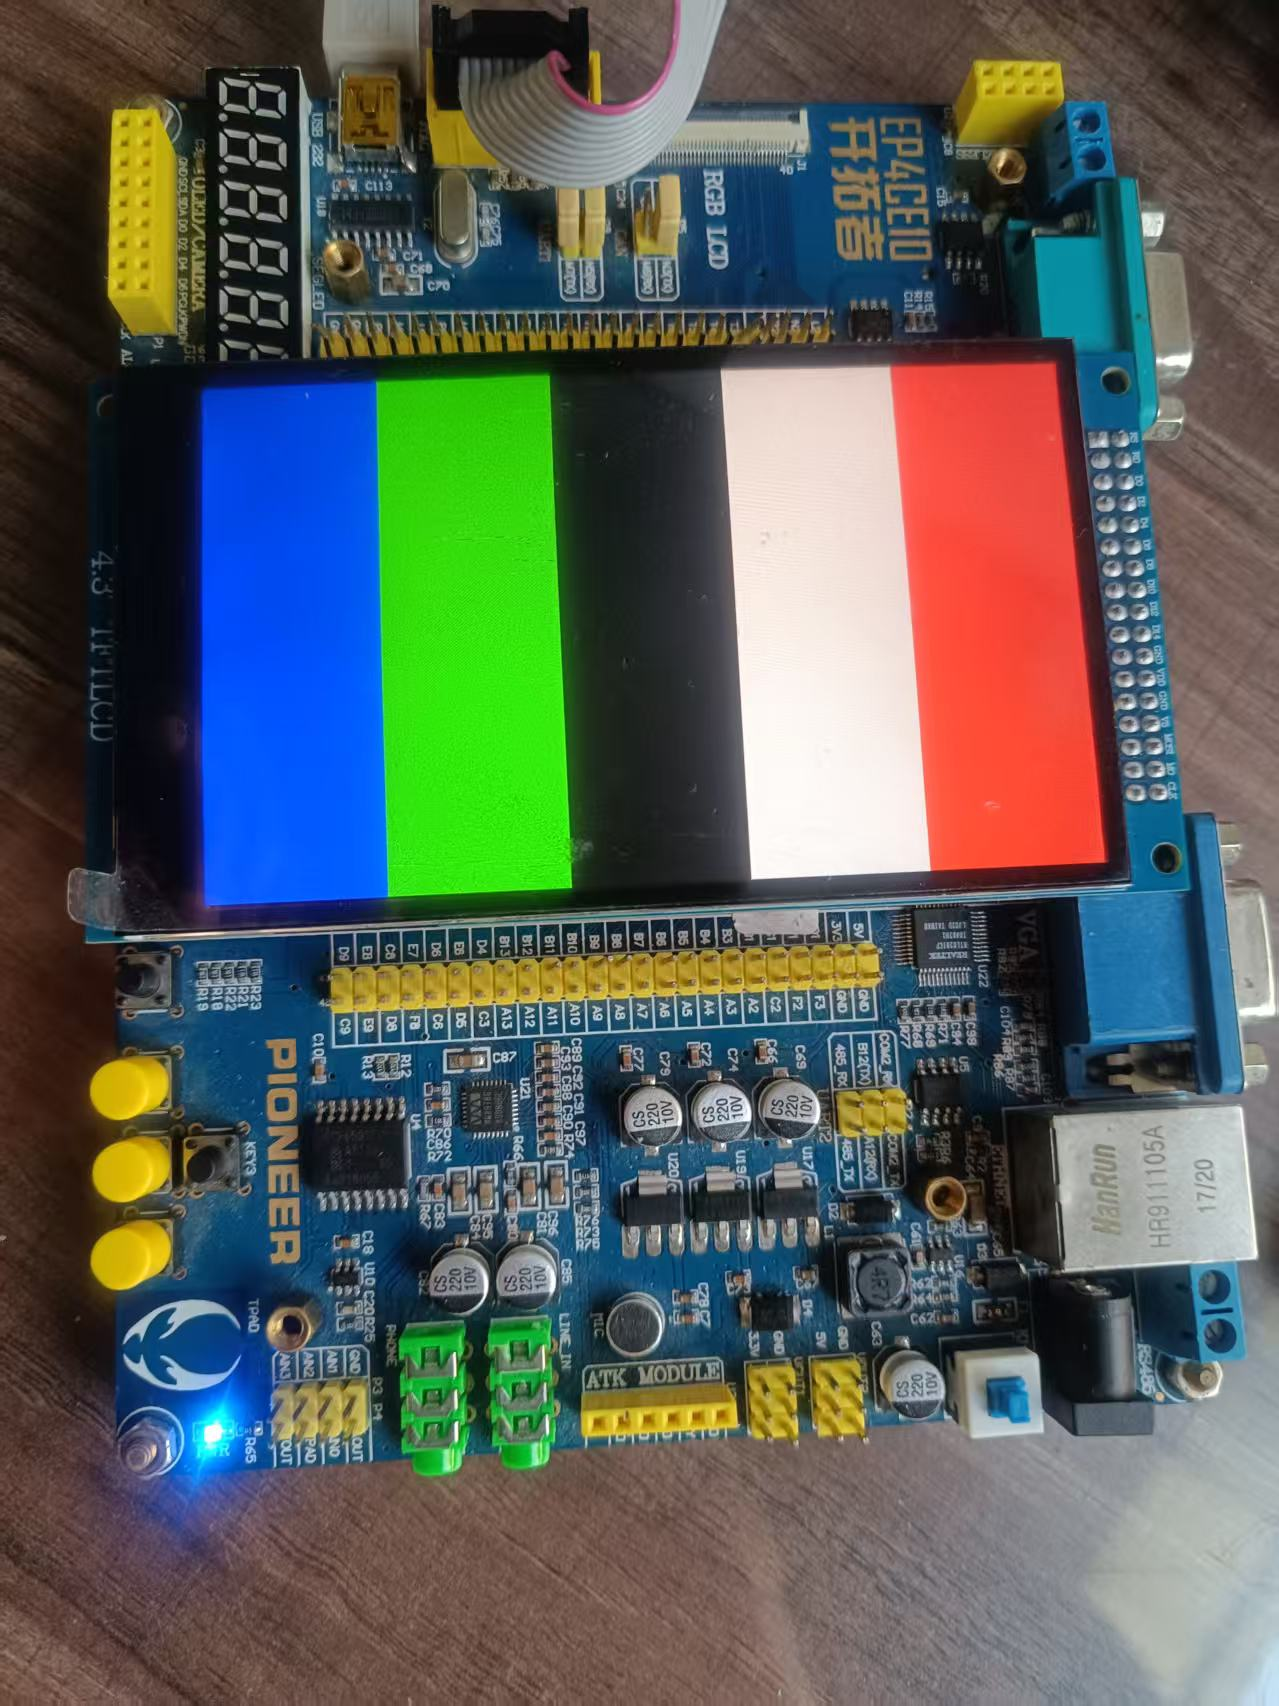
\includegraphics[width=1\textwidth]{figures/003.jpg} % 调整宽度为文本宽度的 80%
        \caption{彩条测试结果} %图片标题
        \label{fig:example} % 图片标签,用于引用
\end{figure}


\section{附录:原程序设计}

附录内主要是业务程序及Qsys配置等,一些公有的IP核、NoisII驱动等内容省略。
\subsection{NoisII软核C程序 main.c}

\begin{lstlisting}[language=C]
#include <stdio.h>
#include "system.h"
#include "io.h"
#include "alt_types.h"
#include "altera_avalon_pio_regs.h"
#include "sys/alt_irq.h"
#include "unistd.h"
#include <string.h>
#include "App/mculcd.h"
#include "sys/alt_cache.h"

extern _lcd_dev lcddev;	//管理LCD重要参数
_lcd_gui lcdgui;

//SDRAM显存的地址
alt_u16 *ram_disp = (alt_u16 *)(SDRAM_BASE + SDRAM_SPAN - 2049000);

int main()
{
    int i,j;
    MY_LCD_Init();              //LCD初始化
    lcdgui.width = lcddev.height;
    lcdgui.height = lcddev.width;
//向sdram中写数据,
   for(i=0;i<lcdgui.width;i++){
      for(j=0;j<lcdgui.height;j++){
        if(j<lcdgui.height/5)
            *(ram_disp++) = 0xf800;     //红色
        else if(j<(lcdgui.height/5*2))
        	*(ram_disp++) = 0xffff;     //白色
        else if(j<(lcdgui.height/5*3))
        	*(ram_disp++) = 0x0;        //黑色
        else if(j<(lcdgui.height/5*4))
            *(ram_disp++) = 0x07e0;     //绿色
        else
            *(ram_disp++) = 0x001f;     //蓝色
        }
   alt_dcache_flush_all();
   }

return 0;
}
\end{lstlisting}

\subsection{Qsys配置}

\begin{figure}[H] % [H] 表示强制当前位置插入
        \centering
        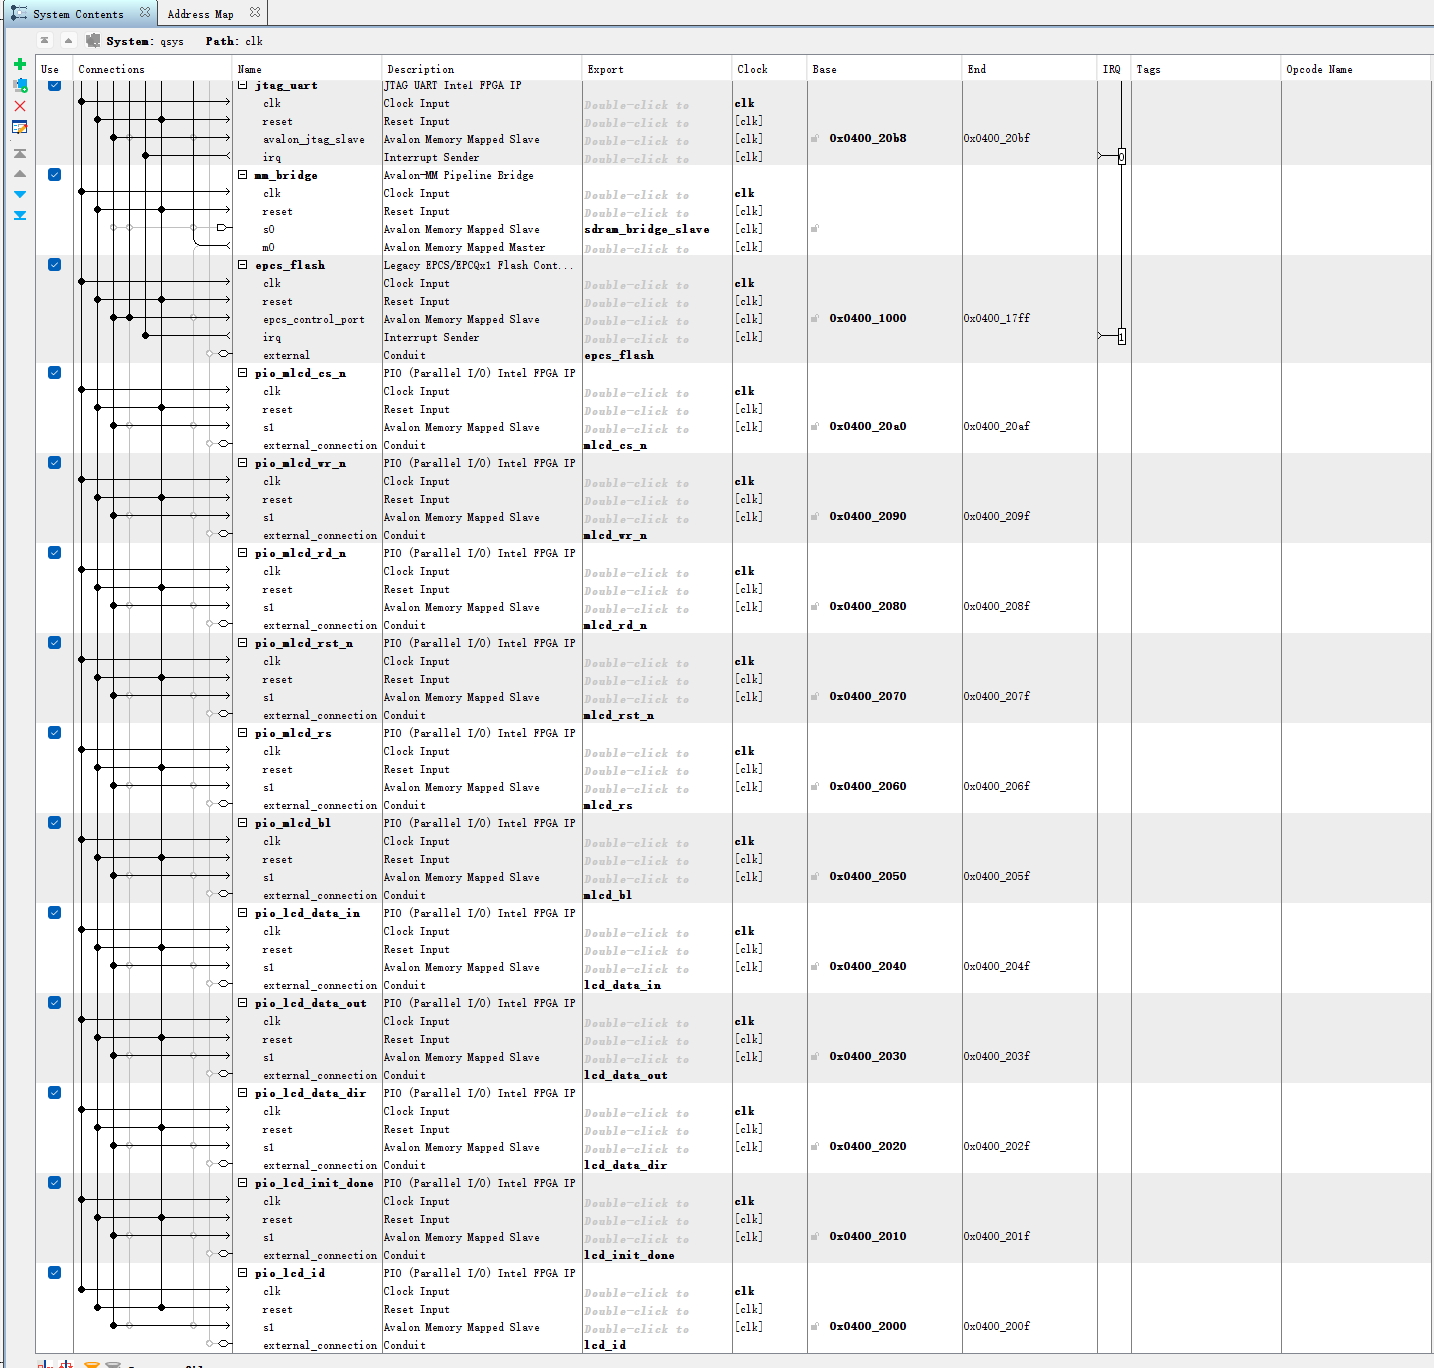
\includegraphics[width=1\textwidth]{figures/004.png} % 调整宽度为文本宽度的 80%
        \caption{Qsys中IP核配置} %图片标题
        \label{fig:example} % 图片标签,用于引用
\end{figure}

\subsection{Verilog顶层文件}

\begin{lstlisting}[language=Verilog]
module Nios_II_colorbar(

    //时钟和复位接口
    input           sys_clk,      //晶振时钟
    input           sys_rst_n,    //按键复位
    
    //SDRAM 接口
    output          sdram_clk,
    output [12:0]   sdram_addr,
    output [ 1:0]   sdram_ba,
    output          sdram_cas_n,
    output          sdram_cke,
    output          sdram_cs_n,
    inout  [15:0]   sdram_dq,
    output [ 1:0]   sdram_dqm,
    output          sdram_ras_n,
    output          sdram_we_n,

    //EPCS Flash 接口
    output          epcs_dclk,
    output          epcs_sce,
    output          epcs_sdo,
    input           epcs_data0,
    
    //LCD接口
    output          lcd_rst    ,  //LCD复位信号
    output          lcd_bl     ,  //LCD背光控制
    output          lcd_de_cs  ,  //LCD RGB:DE  MCU:CS
    output          lcd_vs_rs  ,  //LCD RGB:VS  MCU:RS
    output          lcd_hs_wr  ,  //LCD RGB:HS  MCU:WR
    output          lcd_clk_rd ,  //LCD RGB:CLK MCU:RD
    inout  [15:0]   lcd_data      //LCD DATA
);

//reg define

//wire define
wire        clk_100m_shift;
wire        sys_clk_100m;
wire        clk_50m_pll;
wire        lcd_clk;
wire        pll_locked;
wire        rst_n;

//读写 SDRAM 桥接信号
wire        bridge_write;
wire        bridge_read;  
wire [15:0] bridge_writedata;
wire [15:0] bridge_readdata;
wire [25:0] bridge_address;
wire [ 9:0] bridge_burstcount;
wire        bridge_waitrequest;             
wire        bridge_readdatavalid;

//source_st_fifo信号
wire [9:0]  source_fifo_wrusedw;

//LCD驱动模块接口信号
wire        lcd_data_req;
wire [15:0] lcd_pixel_data;

//LCD初始化完成
wire        lcd_init_done     ;
wire [15:0] lcd_id            ;
wire        mlcd_cs_n_init    ; 
wire        mlcd_wr_n_init    ;
wire        mlcd_rd_n_init    ;
wire        mlcd_rst_n_init   ;
wire        mlcd_rs_init      ;
wire        mlcd_bl_init      ;
wire        mlcd_data_dir_init;
wire [15:0] mlcd_data_out_init;
wire [15:0] mlcd_data_in_init ;

//*****************************************************
//**                    main code
//*****************************************************

assign rst_n = sys_rst_n & pll_locked ;
assign sdram_clk = clk_100m_shift;

//例化锁相环模块
pll u_pll (
    .inclk0                             (sys_clk   ),
    .areset                             (~sys_rst_n),
    .c0                                 (sys_clk_100m),             //QSYS 系统时钟
    .c1                                 (clk_100m_shift),           //SDRAM 时钟
    .c2                                 (clk_50m_pll),              //LCD 驱动时钟
    .locked                             (pll_locked)
    );

//例化QSYS系统
qsys u_qsys(

    //时钟和复位
    .clk_clk                            (sys_clk_100m),
    .reset_reset_n                      (rst_n),
        
    //EPCS  
    .epcs_flash_dclk                    (epcs_dclk ),
    .epcs_flash_sce                     (epcs_sce  ),
    .epcs_flash_sdo                     (epcs_sdo  ),
    .epcs_flash_data0                   (epcs_data0),
        
    //SDRAM 
    .sdram_addr                         (sdram_addr),
    .sdram_ba                           (sdram_ba),
    .sdram_cas_n                        (sdram_cas_n),
    .sdram_cke                          (sdram_cke),
    .sdram_cs_n                         (sdram_cs_n),
    .sdram_dq                           (sdram_dq),
    .sdram_dqm                          (sdram_dqm),
    .sdram_ras_n                        (sdram_ras_n),
    .sdram_we_n                         (sdram_we_n),

    //读写SDRAM的桥     
    .sdram_bridge_slave_waitrequest     (bridge_waitrequest),
    .sdram_bridge_slave_readdata        (bridge_readdata),
    .sdram_bridge_slave_readdatavalid   (bridge_readdatavalid),
    .sdram_bridge_slave_burstcount      (bridge_burstcount),
    .sdram_bridge_slave_writedata       (bridge_writedata),
    .sdram_bridge_slave_address         (bridge_address),
    .sdram_bridge_slave_write           (bridge_write),
    .sdram_bridge_slave_read            (bridge_read),
    .sdram_bridge_slave_byteenable      (2'b11),
    .sdram_bridge_slave_debugaccess     (),
    
    //PIO 输入输出
    .mlcd_cs_n_export                   (mlcd_cs_n_init),            
    .mlcd_wr_n_export                   (mlcd_wr_n_init),            
    .mlcd_rd_n_export                   (mlcd_rd_n_init),            
    .mlcd_rst_n_export                  (mlcd_rst_n_init),            
    .mlcd_rs_export                     (mlcd_rs_init),            
    .mlcd_bl_export                     (mlcd_bl_init),            
    .lcd_data_in_export                 (mlcd_data_in_init),            
    .lcd_data_out_export                (mlcd_data_out_init),            
    .lcd_data_dir_export                (mlcd_data_dir_init),            
    .lcd_init_done_export               (lcd_init_done),           //LCD初始化完成    
    .lcd_id_export                      (lcd_id)                   //LCD ID     
    );
    
//读写 SDRAM 桥 控制模块
sdram_bridge_control u_bridge_ctrl(
    .clk                                (sys_clk_100m),
    .rst_n                              (rst_n & lcd_init_done),
    
    .bridge_write                       (bridge_write),
    .bridge_read                        (bridge_read),
    .bridge_address                     (bridge_address),
    .bridge_burstcount                  (bridge_burstcount), 
    .bridge_waitrequest                 (bridge_waitrequest),
    .bridge_readdatavalid               (bridge_readdatavalid),
    
    .lcd_id                             (lcd_id),
    .source_fifo_wrusedw                (source_fifo_wrusedw)
    );

// FIFO:缓存SDRAM中读出的数据供LCD读取
fifo u_fifo(
    .wrclk                              (sys_clk_100m),
    .rdclk                              (lcd_clk),
                        
    .wrreq                              (bridge_readdatavalid),
    .data                               (bridge_readdata),
    .wrusedw                            (source_fifo_wrusedw),
                        
    .rdreq                              (lcd_data_req),
    .q                                  (lcd_pixel_data),
    .rdempty                            (),
                        
    .aclr                               (~(rst_n & lcd_init_done))
    );

//RGB LCD 和 MCU LCD驱动
lcd_top  u_lcd_top(
    .clk                                (clk_50m_pll),
    .rst_n                              (rst_n & lcd_init_done),
    .pixel_data                         (lcd_pixel_data),
    .pixel_en                           (lcd_data_req),
    .lcd_clk                            (lcd_clk),

    .lcd_rst                            (lcd_rst),
    .lcd_bl                             (lcd_bl),
    .lcd_de_cs                          (lcd_de_cs),
    .lcd_vs_rs                          (lcd_vs_rs),
    .lcd_hs_wr                          (lcd_hs_wr),
    .lcd_clk_rd                         (lcd_clk_rd),
    .lcd_data                           (lcd_data),
                
    .mlcd_cs_n_init                     (mlcd_cs_n_init),
    .mlcd_wr_n_init                     (mlcd_wr_n_init),
    .mlcd_rd_n_init                     (mlcd_rd_n_init),
    .mlcd_rst_n_init                    (mlcd_rst_n_init),
    .mlcd_rs_init                       (mlcd_rs_init),
    .mlcd_bl_init                       (mlcd_bl_init),
    .mlcd_data_dir_init                 (mlcd_data_dir_init),
    .mlcd_data_out_init                 (mlcd_data_out_init),
    .mlcd_data_in_init                  (mlcd_data_in_init ),
    .lcd_init_done                      (lcd_init_done),
    .lcd_id                             (lcd_id)
    );

endmodule 


\end{lstlisting}

\subsection{Verilog重要驱动1:LCD驱动}

\begin{lstlisting}[language=Verilog]
//****************************************Copyright (c)***********************************//
//技术支持:www.openedv.com
//淘宝店铺:http://openedv.taobao.com 
//关注微信公众平台微信号:"正点原子",免费获取FPGA & STM32资料。
//版权所有,盗版必究。
//Copyright(C) 正点原子 2018-2028
//All rights reserved                                  
//----------------------------------------------------------------------------------------
// File name:           mlcd_driver
// Last modified Date:  2018/1/30 11:12:36
// Last Version:        V1.1
// Descriptions:        MCU LCD驱动
//----------------------------------------------------------------------------------------
// Created by:          正点原子
// Created date:        2018/1/29 10:55:56
// Version:             V1.0
// Descriptions:        The original version
//
//----------------------------------------------------------------------------------------
// Modified by:         正点原子
// Modified date:       2018/8/15 14:23:12
// Version:             V1.1
// Descriptions:        Intel8080总线
//
//----------------------------------------------------------------------------------------
//****************************************************************************************//

module mlcd_driver(
    input         clk       ,    //时钟
    input         rst_n     ,    //复位,低电平有效
    output        mlcd_bl   ,    //MCU LCD 背光控制信号 
    output        mlcd_cs   ,    //MCU LCD 片选信号 
    output        mlcd_rst  ,    //MCU LCD 复位信号
    output        mlcd_wr   ,    //MCU LCD 写使能信号
    output        mlcd_rd   ,    //MCU LCD 读使能信号
    output        mlcd_rs   ,    //MCU LCD 指令/数据控制信号
    output [15:0] mlcd_data ,    //MCU LCD 双向数据总线
    
    input         lcd_init_done, //LCD初始化完成
    input  [15:0] lcd_id    ,    //LCD ID
    input  [15:0] pixel_data,    //从fifo中读出的数据    
    output  reg   rd_en          //fifo读使能信号
    );
    
//parameter define     
parameter  idle = 2'd0;
parameter  step1 = 2'd1;
parameter  step2 = 2'd2;
parameter  step3 = 2'd3;

//reg define
reg        lcd_done_d0;
reg        lcd_done_d1;
reg [15:0] lcd_id_r;

reg [10:0] lcd_height;
reg [10:0] lcd_width;

reg        wr_r; 
reg        rd_r;
reg        rs_r;
reg [15:0] data_r;

reg [2:0]  wr_step;
reg [10:0] h_cnt;
reg [10:0] v_cnt; 
reg [10:0] h_blank_cnt;
reg [10:0] v_blank_cnt;

//wire define
wire       pos_lcd_done;

//*****************************************************
//**                    main code
//*****************************************************  

assign mlcd_bl   = 1'b1;        //设置屏幕背光为最亮
assign mlcd_cs   = 1'b0;        //片选信号低电平有效
assign mlcd_rst  = 1'b1;        //初始化完成后,LCD不复位
assign mlcd_wr   = wr_r;        //LCD写信号
assign mlcd_rd   = rd_r;        //LCD读信号
assign mlcd_rs   = rs_r;        //LCD指令/数据控制信号
assign mlcd_data = data_r;      //LCD数据线

assign pos_lcd_done = ~lcd_done_d1 & lcd_done_d0;

//lcd_init_done上升沿
always@(posedge clk or negedge rst_n) begin
    if(!rst_n) begin
        lcd_done_d0 <= 1'b0;
        lcd_done_d1 <= 1'b0;
    end
    else begin
        lcd_done_d0 <= lcd_init_done;
        lcd_done_d1 <= lcd_done_d0;
    end        
end    

always@(posedge clk or negedge rst_n) begin
    if(!rst_n) 
        lcd_id_r <= 16'd0;
    else if(pos_lcd_done)
        lcd_id_r <= lcd_id;
end

//利用状态机向LCD控制器写指令及数据
always@(posedge clk or negedge rst_n) begin
    if(!rst_n) begin
        wr_r        <= 1'b1;
        rd_r        <= 1'b1;
        rs_r        <= 1'b0;
        data_r      <= 16'd0;           
        rd_en       <= 1'b0;
        lcd_height  <= 11'b0;
        lcd_width   <= 11'b0;
        h_cnt       <= 11'd0;
        v_cnt       <= 11'b0;
        h_blank_cnt <= 11'b0;
        v_blank_cnt <= 11'b0;
        wr_step     <= idle;
    end
    else begin
        case(wr_step)      
            idle: begin
                rd_r     <= 1'b1; 
                wr_r     <= 1'b1;
                rd_en    <= 1'b0;   
                if(lcd_done_d1) begin   
                    wr_step <= step1; 
                    case(lcd_id_r)           //根据LCD ID,选择不同的寄存器指令与分辨率
                        16'h9341 : begin
                            lcd_width   <= 11'd320-1'b1;
                            lcd_height  <= 11'd240-1'b1;
                            h_blank_cnt <= 30;
                            v_blank_cnt <= 10;
                        end    
                        16'h5310 : begin
                            lcd_width   <= 11'd480-1'b1;
                            lcd_height  <= 11'd320-1'b1;
                            h_blank_cnt <= 80;
                            v_blank_cnt <= 45;
                        end    
                        16'h5510 : begin
                            lcd_width   <= 11'd800-1'b1;
                            lcd_height  <= 11'd480-1'b1;
                            h_blank_cnt <= 11'd200;
                            v_blank_cnt <= 11'd15;
                        end                      
                        16'h1963 : begin
                            lcd_height  <= 11'd800-1'b1;
                            lcd_width   <= 11'd480-1'b1;
                            h_blank_cnt <= 11'd200;
                            v_blank_cnt <= 11'd15;
                        end       
                        default : wr_step <= idle;
                    endcase     
                end 
                else
                    wr_step <= idle;
            end
            step1: begin                               //发送写GRAM指令
                wr_r <= 1'b0;
                rs_r <= 1'b0;    
                if(lcd_id_r == 16'h5510)
                    data_r <= 16'h2c00;              
                else
                    data_r <= 16'h002c;    
                if(wr_r == 1'b0) begin
                    wr_r <= 1'b1;
                    wr_step <= step2;
                end
            end
            step2 : begin
                wr_r <= 1'b1;
                h_cnt <= h_cnt + 1'b1;
                if(h_cnt == lcd_width + h_blank_cnt + 1'b1) begin
                    h_cnt <= 11'd0;
                    v_cnt <= v_cnt + 1'b1;
                    if(v_cnt == lcd_height + v_blank_cnt + 1'b1) begin
                        v_cnt <= 11'd0;
                        wr_step <= idle;
                    end                        
                end  
                if(v_cnt >= v_blank_cnt && v_cnt <= (lcd_height + v_blank_cnt)) begin
                    if(h_cnt >= h_blank_cnt && h_cnt <= (lcd_width + h_blank_cnt))
                        wr_step <= step3;  
                    if(h_cnt == h_blank_cnt - 1'b1)    //提前拉高fifo读使能信号
                        rd_en <= 1'b1;
                    else
                        rd_en <= 1'b0;                           
                end  
                else
                    rd_en <= 1'b0;     
            end
            step3: begin                               //写像素数据
                wr_r <= 1'b0;
                rs_r <= 1'b1;                                       
                data_r <= pixel_data;                                        
                wr_step <= step2;
                if(h_cnt == lcd_width + h_blank_cnt + 1'b1)
                    rd_en <= 1'b0;
                else    
                    rd_en <= 1'b1;
            end
        endcase     
    end
end   

endmodule 



\end{lstlisting}

\subsection{Verilog重要驱动2:SDRAM控制器}

\begin{lstlisting}[language=Verilog]
module sdram_bridge_control(
    input               clk                   ,
    input               rst_n                 ,
    
    output  reg         bridge_write          ,
    output  reg         bridge_read           ,
    output  reg  [25:0] bridge_address        ,
    output  reg  [9:0]  bridge_burstcount     ,
    input               bridge_waitrequest    ,
    input               bridge_readdatavalid  ,
    
    input        [15:0] lcd_id                ,
    input        [ 9:0] source_fifo_wrusedw
    );

//parameter define

//SDRAM 存储容量 = 2^13(row)*2^9(col)*4(bank)*2(byte)
parameter SDRAM_SPAN = 33554432;

//LCD存储图像地址参数设置(800*480)
parameter  sdram_addr_start   = SDRAM_SPAN - 2048000 - 1000;     //sdram显存起始地址;
parameter  sdram_addr_end_320_240  = sdram_addr_start + 153600;  //结束地址(320*240)
parameter  sdram_addr_end_480_272  = sdram_addr_start + 261120;  //结束地址(480*272)
parameter  sdram_addr_end_480_320  = sdram_addr_start + 307200;  //结束地址(480*320)
parameter  sdram_addr_end_800_480  = sdram_addr_start + 768000;  //结束地址(800*480)
parameter  sdram_addr_end_1024_600 = sdram_addr_start + 1228800; //结束地址(1024*600)
parameter  sdram_addr_end_1280_800 = sdram_addr_start + 2048000; //结束地址(1280*800)
parameter  burstcount            = 10'd512;                      //SDRAM 突发长度
parameter  burst_addr            = 11'd1024 ;                    //一次突发的地址长度
parameter  usedw_wr              = 512;                          //读fifo的数据深度

//reg define
reg  [25:0] address_rd;       //读fifo端读取数据的sdram地址
reg  [9:0]  cnt_burst;        //计数一次突发读数据过程中已读取的个数
reg         step;             //step
reg         step_1;
reg  [25:0] sdram_addr_end;   //sdram显存结束地址

//wire define 
wire burst_start;             //开始突发标志

//*****************************************************
//**                    main code
//*****************************************************

//采集step上升沿信号,标志着突发传输指令已发出
assign burst_start = (~step_1 ) & step;

//寄存step信号,用于边沿捕获
always @ (posedge clk  or negedge rst_n ) begin 
    if(!rst_n ) 
        step_1 <= 1'b0;
    else    
        step_1 <=  step;  
end

always @ (*) begin
    case(lcd_id)
        16'h4342 : sdram_addr_end = sdram_addr_end_480_272 ;
        16'h7084 : sdram_addr_end = sdram_addr_end_800_480 ;
        16'h7016 : sdram_addr_end = sdram_addr_end_1024_600;
        16'h1018 : sdram_addr_end = sdram_addr_end_1280_800;
        16'h9341 : sdram_addr_end = sdram_addr_end_320_240 ;
        16'h5310 : sdram_addr_end = sdram_addr_end_480_320 ;
        16'h5510 : sdram_addr_end = sdram_addr_end_480_320 ;
        16'h1963 : sdram_addr_end = sdram_addr_end_480_320 ;
    default  : sdram_addr_end = sdram_addr_end_480_272 ;
    endcase 
end

//读SDRAM的地址
always @ (posedge clk or negedge rst_n ) begin
    if(!rst_n )
        address_rd <= sdram_addr_start;
    else if (address_rd == sdram_addr_end) 
            address_rd <= sdram_addr_start;
    else if (burst_start)
        address_rd <= address_rd + burst_addr; 
end

//计数突发读出的数据个数
always @ (posedge clk or negedge rst_n) begin
    if(!rst_n)
        cnt_burst <= 10'b0;
    else if (cnt_burst == burstcount) 
        cnt_burst <= 10'b0;
    else if (bridge_readdatavalid)
        cnt_burst <= cnt_burst + 1'b1;
end 

//fifo中的数据量低于512时,从sdram中读数据
always @ (posedge clk or negedge rst_n) begin
    if(!rst_n) begin
        step                <= 1'b0;   
        bridge_read         <= 1'b0;         
        bridge_write        <= 1'b0;
        bridge_address      <= 26'b0;
        bridge_burstcount   <= 10'b0;
    end 
    else if((! bridge_waitrequest) && (source_fifo_wrusedw < usedw_wr) 
            &&(cnt_burst == 10'd0) ) begin  //从sdram读数据
        case(step)    
            1'b0: begin 
                step                <= 1'b1;
                bridge_read         <= 1'b1;   
                bridge_write        <= 1'b0;
                bridge_address      <= address_rd;
                bridge_burstcount   <= burstcount;
            end 
            1'b1: begin
                bridge_read       <= 1'b0;   
                bridge_address    <= 26'b0;
                bridge_burstcount <= 10'b0;
            end
        default: ;         
        endcase   
    end 
    else if (cnt_burst == burstcount)  
        step <= 1'b0;
end

endmodule       


\end{lstlisting}

\end{document}